% arara: pdflatex: { synctex: yes }
% arara: makeindex: { style: ctuthesis }
% arara: bibtex

% The class takes all the key=value arguments that \ctusetup does,
% and a couple more: draft and oneside
\documentclass[twoside]{ctuthesis}

\ctusetup{
	preprint = \ctuverlog,
	mainlanguage = english,
	titlelanguage = english,
%	mainlanguage = czech,
	otherlanguages = {slovak,english},
	title-czech = {Detekce dronů pomocí neuronových sítí z kombinovaných dat RGB kamery a LIDARu},
	title-english = {Drone detection using neural networks from combined RGB camera and LiDAR data},
	%subtitle-czech = {Cesta do tajů kdovíčeho},
%	subtitle-english = {Journey to the who-knows-what wondeland},
	doctype = B,
	faculty = F3,
	department-czech = {Katedra kybernetiky},
	department-english = {Department of Cybernetics},
	author = {Adam Škuta},
	supervisor = {Ing. Matouš Vrba},
	supervisor-address = {Ústav X, \\ Uliční 5, \\ Praha 99},
	supervisor-specialist = {},
	fieldofstudy-english = {Cybernetics and Robotics},
	fieldofstudy-czech = {Kybernetika a Robotika},
	keywords-czech = {Dron, Konvolučná neurónová sieť, Detekcia, LiDAR, Riedka hĺbková mapa},
	keywords-english = {Drone, Convolutional neural network, Detection, LiDAR, Sparse depthmap},
	day = 4,
	month = 1,
	year = 2022,
	specification-file = {zav_prace.pdf},
	front-specification = true,
%	front-list-of-figures = true,
%	front-list-of-tables = true,
%	monochrome = true,
%	layout-short = true,
}

\ctuprocess

\addto\ctucaptionsczech{%
	\def\supervisorname{Vedoucí}%
	\def\subfieldofstudyname{Studijní program}%
}

\ctutemplateset{maketitle twocolumn default}{
	\begin{twocolumnfrontmatterpage}
		\ctutemplate{twocolumn.thanks}
		\ctutemplate{twocolumn.declaration}
		\ctutemplate{twocolumn.abstract.in.titlelanguage}
		\ctutemplate{twocolumn.abstract.in.secondlanguage}
		\ctutemplate{twocolumn.tableofcontents}
		\ctutemplate{twocolumn.listoffigures}
	\end{twocolumnfrontmatterpage}
}

% Theorem declarations, this is the reasonable default, anybody can do what they wish.
% If you prefer theorems in italics rather than slanted, use \theoremstyle{plainit}
\theoremstyle{plain}
\newtheorem{theorem}{Theorem}[chapter]
\newtheorem{corollary}[theorem]{Corollary}
\newtheorem{lemma}[theorem]{Lemma}
\newtheorem{proposition}[theorem]{Proposition}

\theoremstyle{definition}
\newtheorem{definition}[theorem]{Definition}
\newtheorem{example}[theorem]{Example}
\newtheorem{conjecture}[theorem]{Conjecture}

\theoremstyle{note}
\newtheorem*{remark*}{Remark}
\newtheorem{remark}[theorem]{Remark}

\setlength{\parskip}{5ex plus 0.2ex minus 0.2ex}
\graphicspath{{figures/}}

% Abstract in Czech
\begin{abstract-czech}
	Detekcia dron pomocou neurónových sietí z kombinovaných dát RGB kamery a Light Detecting And Ranging (LiDARu) je popísaná v tejto práci. Viacero spôsobov kombinácie RGB kamery a LiDARu do Red Green Blue Depth (RGBD) obrázkov je prezentovaných. Samotná detekcia dron je realizovaná pomocou konvolučnej neurónovej siete. Všetky metódy sú natrénované a otestované a následné výsledky sú porovnané s čistou RGB kamerou. Dáta používané v tejto práci boli vygenerované pomocou viacerých virtuálnych prostredí. Výsledky dokazujú, že v niektorých prípadoch RGBD metódy produkujú lepšie výsledky oproti RGB kamere v kontexte detekcie dronov. Budúca práca preto predstavuje ďaľšiu zaujímavú štúdiu.
\end{abstract-czech}

% Abstract in English
\begin{abstract-english}
Detection of drones using neural networks from combined RGB and Light Detecting And Ranging (LiDAR) data is tackled in this thesis. Multiple approaches for RGB and LiDAR data fusion into Red Green Blue Depth (RGBD) data are presented. The detection of the drone is realized via a convolutional neural network. All methods are trained and tested and the results are compared with a detection approach utilizing only RGB images. The dataset used in this thesis was generated using multiple Simulated environments. The results show that there is a difference between RGBD and RGB approaches and that in some specific scenarios, RGBD approaches provide an advantage over using RGB only in drone detection. Further work on these methods is therefore a worthwhile study.
\end{abstract-english}

% Acknowledgements / Podekovani
\begin{thanks}
I would like to express my utmost gratitude to my supervisor Ing. Matouš Vrba for his guidance and great support during my time writing this thesis.\\
\\
I would also like to thank my parents and friends for their huge support and help.
\end{thanks}

% Declaration / Prohlaseni
\begin{declaration}
Prehlasujem, že som predloženú prácu vypracoval samostatne , a že som uviedol všetku použitú literatúru.

V Praze, \ctufield{day}.~\monthinlanguage{title}~\ctufield{year}
\end{declaration}

% Only for testing purposes
\listfiles
\usepackage[pagewise]{lineno}
\usepackage{lipsum,blindtext}
\usepackage{mathrsfs} % provides \mathscr used in the ridiculous examples
\usepackage{todonotes}
\usepackage{amsmath}
\usepackage{xspace}
\usepackage{caption}
\usepackage{subcaption}
\usepackage{multirow}
\usepackage{hyperref}
\usepackage{pdfpages}
\usepackage{siunitx}

\begin{document}

\maketitle
\chapter{Introduction}
In this thesis, drone detection using neural networks and combined data from an RGB camera and a Light Detection And Ranging (LiDAR) sensor is studied. With the recent development of drone technology, drones have become more readily available to the public and can only be expected to rise in popularity in the future. Drone detection is an important problem to tackle when it comes to tasks such as interception of uncooperative drones \cite{cite:1} or localization of drones in swarm \cite{cite:2} \cite{cite:3}. The methods presented in this thesis are intended for the relative localization of both cooperating and non-cooperating drones. Compared to absolute localization methods, relative localization does not need to rely on pre-existing ground infrastructure and can be used in more environments. LiDAR sensor has been utilized on drones on multiple occasions \cite{cite:4} \cite{9553611} \cite{9554023} and an RGB camera provides an easily accessible, cheap and lightweight sensor. Therefore, a fusion of data retrieved from both sensors and its impact on the overall drone detection problem is an interesting problem to tackle. The results can be useful for occasions where a drone is already equipped with a LiDAR sensor. Or they can provide further clarification, whether the addition of LiDAR sensor into the drone detection problem provides any advantage.\\
\\
The goal of this thesis was to examine whether usage of LiDAR data coupled with RGB images from camera is useful for the localization of drones in contrast to the usage of image data alone. The LiDAR and RGB camera were mounted on top of the observer drone, which took pictures and pointclouds of the target drone. All the measurements were taken inside a virtual environment, with a realistic drone and sensor simulation. The dataset was then processed and used as the input for training and testing a convolutional neural network for the object detection as can be seen in \autoref{fig:intro}. The preprocessing was as follows:
\begin{itemize}
	\item coordinate transformation for the non-matching coordinate systems,
	\item projection of 3D points into a 2D image,
	\item utilizing different processing methods on sparse LiDAR depthmap to make it denser,
	\item fusing RGB images and LiDAR data into Red Green Blue Depth (RGBD) images.
\end{itemize}
The output metrics were then compared with the RGB trained convolutional neural network metrics.
\begin{figure}
	\centering
	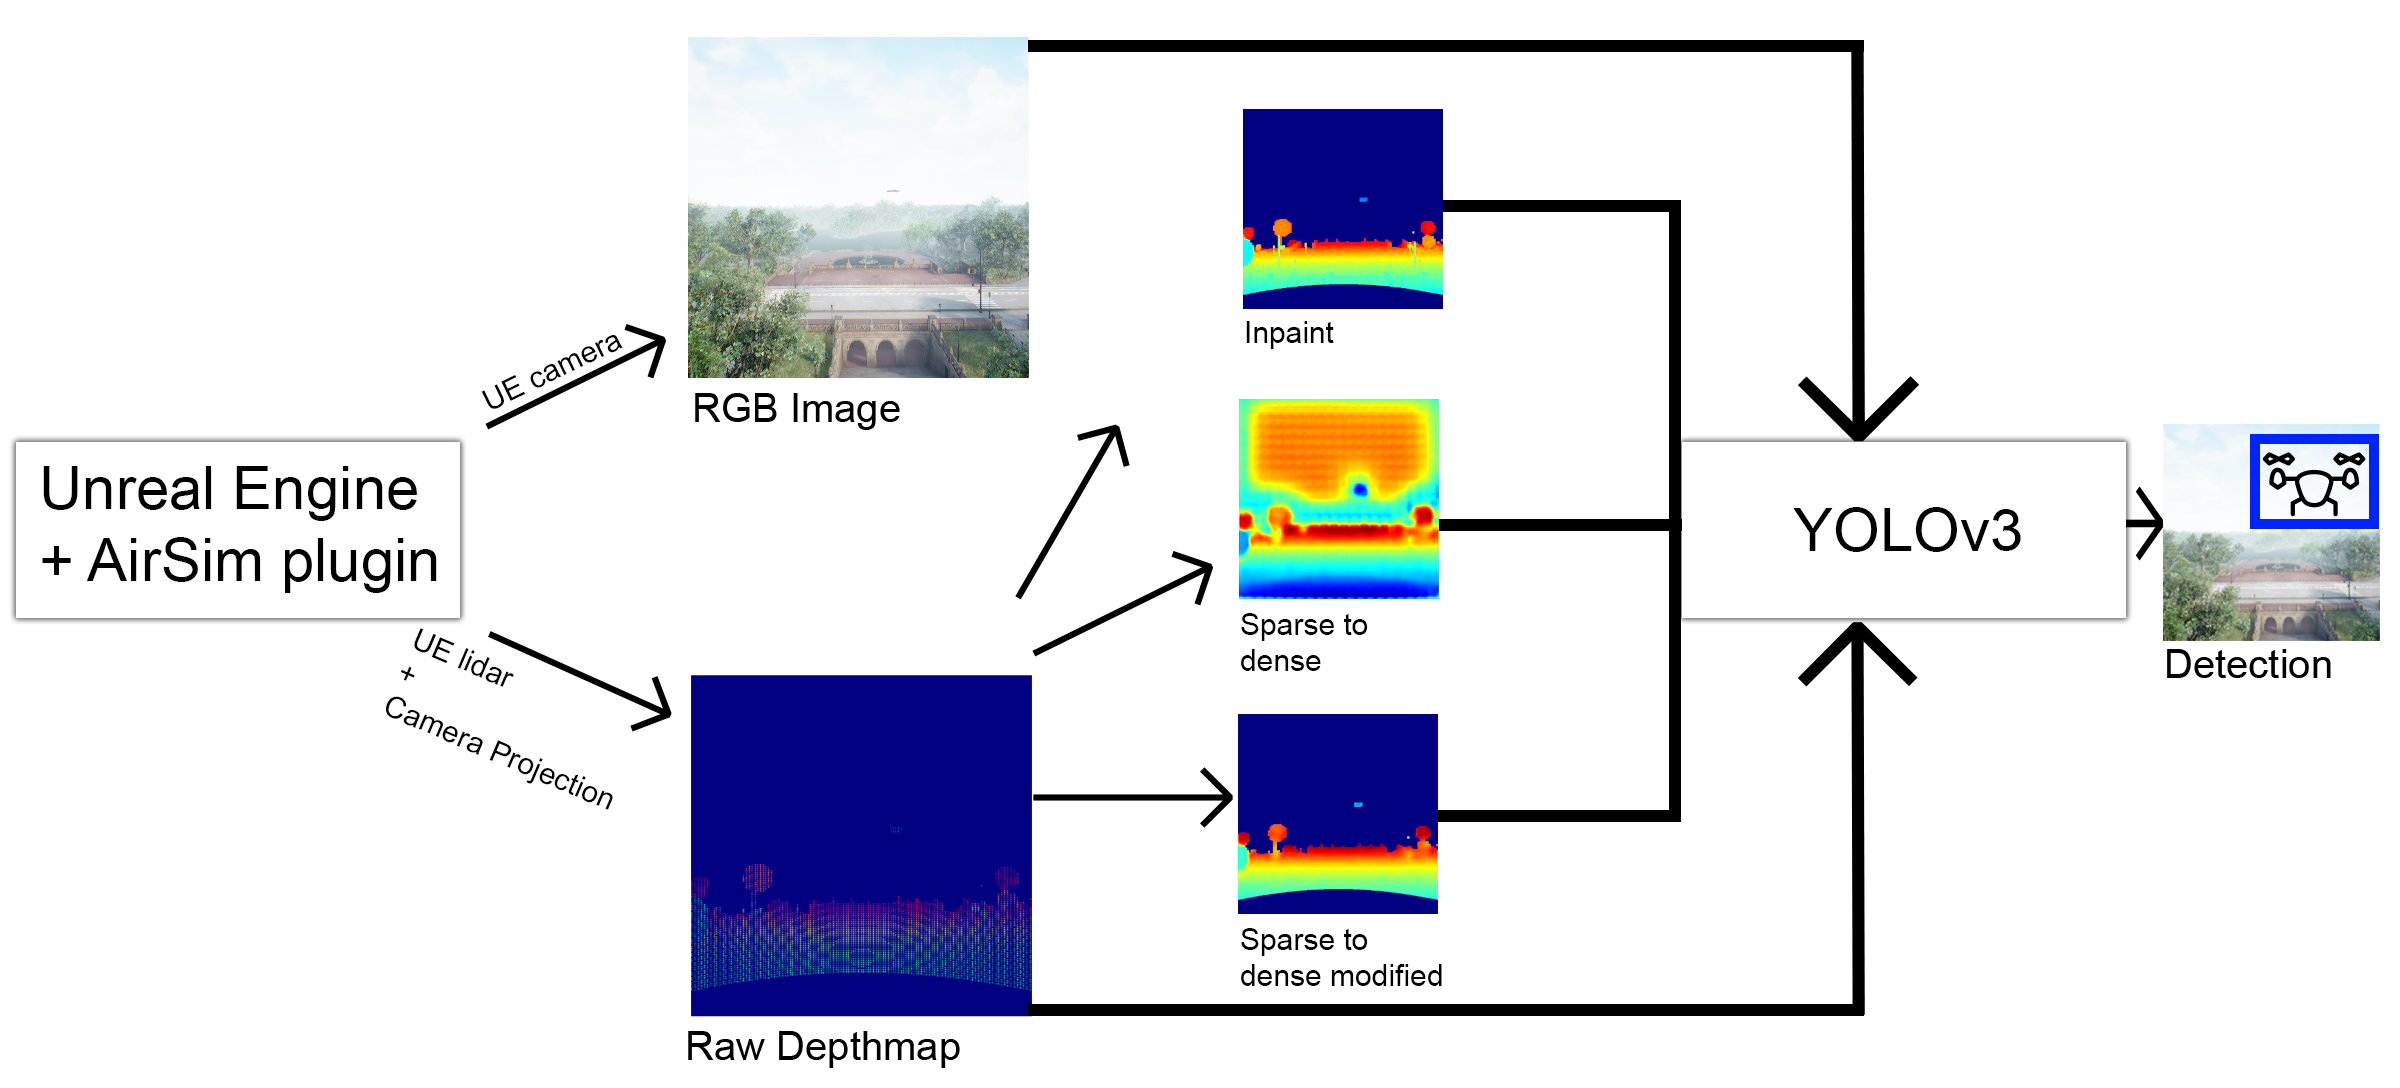
\includegraphics[width=\textwidth]{detection_schema.png}
	\caption{Schema of the process.}
	\label{fig:intro}
\end{figure}
\section{Related Work}
Solving the problem of drone detection has been tackled in different ways. They mostly differ with the sensors that are utilized or by placing markers on flying drones.
\begin{itemize}
	\item \textbf{static sensors} current state-of-the-art drone detection techniques utilizing static sensors such as radars, acoustic sensors or Wi-Fi rely on pre-existing infrastructure. According to the results presented in \cite{8337899}, radar technology faces multiple challenges when detecting smaller aircrafts such as drones because of their small size and high altitude of their flight but shows promising results. When it comes to accoustic sensors, sound of the drone can be a very good source of information but depends heavily on the ambient sound of its environment \cite{8337899}. In \cite{drone-det-wifi}, the authors presented a method for drone detection using Wi-FI packets that are sent between the drone and its user. This method relies on the fact that most commercially available drones utilize Wi-Fi packets when it comes to communication with the end user. However, only the presence of the drone in the vicinity of the sensor can be detected using this method and not its exact location, which is crucial for most multi-robotic tasks.
	\item \textbf{marker-based detection} some of the relative localization techniques utilize a set of markers that are placed on a target. In \cite{holter2020relative}, an observer drone detects and localizes drones equipped with markers using a spherical camera with a $360^\circ$ field of view. This system is applied in real-time and provides accurate localization with $\SI{4}{\centi \metre}$ precision. Another approach is provided in \cite{8651535}, where ultra-violet emitters are equipped on a drone and serve as detection markers for detection using an ultra-violet camera sensor. This approach proved to be successful in real-life situations. The downside of utilizing visual markers on target drones is that a hardware modification of the target drone is required. Therefore, this approach is not applicable to all situations, especially when the target drone is not cooperating.
	\item \textbf{convolutional neural networks} due to its speed, accuracy and advancements, object detection convolutional neural networks have become a popular technique for relative drone detection such as YOLOv3 \cite{redmon2018yolov3}, CenterNet \cite{zhou2019objects}, RetinaNet \cite{lin2018focal} and Faster R-CNN \cite{ren2016faster}. One approach of using a convolutional neural network is described in \cite{ali2018yolo3d}. This approach is similar to the approach presented in this thesis in the sense that it fuses RGB and LiDAR data and use them as input into the modified YOLOv2 \cite{redmon2016yolo9000} convolutional neural network. This approach represents the LiDAR pointcloud as a birds-eye-view map and outputs 7 degrees of freedom, which includes the position, size and rotation of the bounding box for the detected objects. Another approach described in \cite{8988144} uses a convolutional neural network for the use of relative micro aerial vehicle detection. This approach uses tiny-YOLO architecture \cite{redmon2016yolo9000} and estimates the distance of the detected vehicle from the size of its bounding box. The results prove to be applicable in real-world scenarios. For this thesis, a YOLOv3 architecture is utilized due to its speed and simplicity, making the utilization of the LiDAR data easier,
	\item \textbf{dense depthmap} a LiDAR produces sparse depthmaps, which are not always satisfactory for further use. Therefore, ways to denser the sparse depthmaps have been explored. In \cite{zhang2020listereo} dense depthmaps are generated by combining LiDAR with Stereo Imagery using a convolutional neural network with a self-supervised training process. This method shows that the method used can create dense depthmaps even from low-resolution LiDAR measurements and therefore reduce the cost by utilizing a low-resolution LiDAR sensor. Another method is described in \cite{ma2018sparsetodense}. It uses sparse depthmaps combined with RGB images as an input to the convolutional neural network to create a dense depthmap. This method is used in the thesis. In \cite{cite:5} an image inpainting method is utilized, which fills in unknown pixel values based on the neighbouring known pixel values. It is usually used for inpainting RGB or grayscale images, but it can be used for sparse depthmaps as well and is used in this thesis.
\end{itemize}
\section{Problem Statement}
An RGB camera and a LiDAR sensor are assumed to be mounted on an observer drone so that their fields of view overlap. The transformation between coordinate frames of the LiDAR and the camera must be known. The target drone is located in a range of 0.9 meters to 100 meters and has length, width and height dimensions of 0.6, 1.0 and 0.3 meters, respectively. The drone is located in the field of view of both sensors and is not obstructed by any other object. The location of the target drone on the image is required to be determined from the data obtained from both sensors.
\chapter{Methodology}
In this chapter, five different approaches to the detection problem were tackled:
\begin{itemize}
	\item RGB-only
	\item Sparse-to-dense RGBD
	\item Sparse-to-dense modified RGBD
	\item Inpaint RGBD
	\item Raw RGBD
\end{itemize}
The baseline approach in this thesis is to use RGB image and use it as an input into the YOLOv3 \cite{redmon2018yolov3} convolutional neural network for drone detection.\\
\\
The second approach utilizes the Sparse-to-dense convolutional neural network \cite{ma2018sparsetodense}, which takes sparse LiDAR depthmap and RGB image as an input and outputs dense LiDAR depthmap. The neural network is pre-trained and its output is concatenated with RGB images and used as an input into the YOLOv3  for drone detection\\
\\
Another approach is to use the output of Sparse-to-dense network and further process the data, eliminating sections of the depth image that are very sparse and using the output concatenated with RGB images to use as input for YOLOv3.\\
\\
A separate approach is to use the inpainting method from the OpenCV Python library, which takes sparse LiDAR depthmap and fills in unknown values based on the nearby known values, outputting dense depthmap. The output of the inpainting method is further processed to filter inpainted values that are very far from known values and concatenated with RGB images to use as an input into YOLOv3.\\
\\
The final approach is to concatenate sparse LiDAR depthmap with RGB images and use it as an input into YOLOv3.\\
\\
A video game engine Unreal Engine\footnote{\url{https://www.unrealengine.com}}paired with plugin AirSim\footnote{\url{https://microsoft.github.io/AirSim/}} is used for simulating real-life environments and for generating the dataset.
\section{Sparse-to-dense} \label{s2d}
Sparse-to-dense \cite{ma2018sparsetodense} is a convolutional neural network with an implementation in PyTorch publicly available. The input into the network is a sparse depthmap and an RGB image and the output is a dense depthmap.  The sparse depthmap is a matrix with few values that have known depth value and the rest are unknowns. In the dense depthmap every value is known. The size of the network is modifiable and can be chosen as a meta-parameter.
\begin{figure}
	\caption[Example of different network architectures available.]{Example of different network architectures available. Taken from \cite{ma2018sparsetodense}.}
	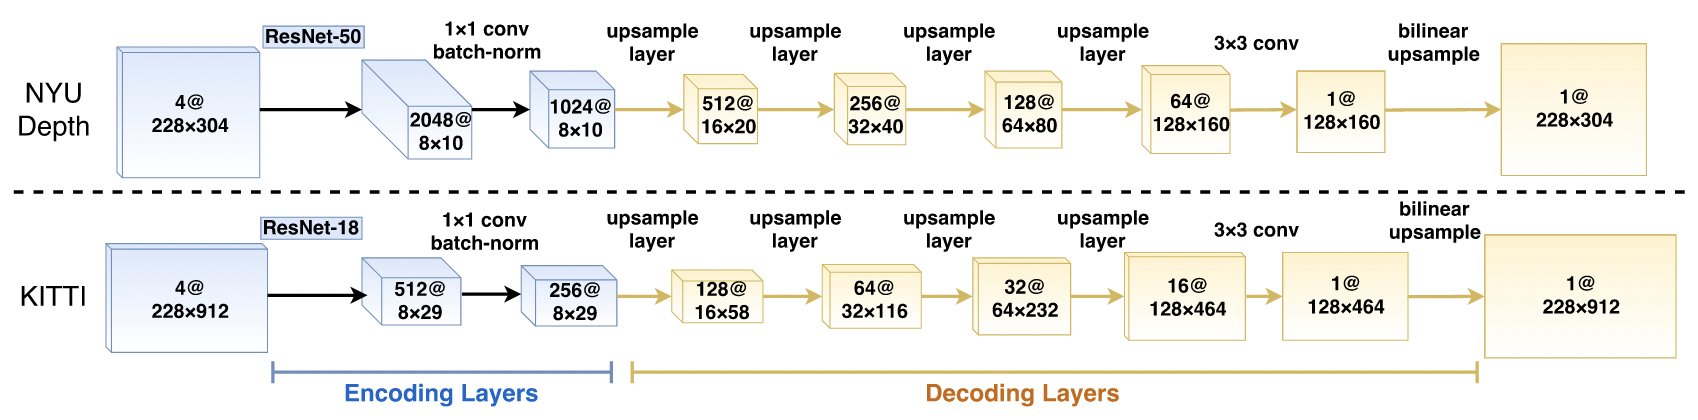
\includegraphics[width=\textwidth]{sparse2dense.png}
	\centering
	\label{fig:s2d_model}
\end{figure}
For the encoding layers, a ResNet-50 or ResNet-18 can be chosen depending on the size of the input image as can be seen in \autoref{fig:s2d_model}. The decoding layers consist of 4 upsampling layers and a deconvolutional layer with either stride 2 or 3 or uprojection layer or upconvolutional layer as a choice for training. The loss function used for backpropagation is the least absolute deviations error also known as $L_1$ error:
\begin{equation}
	L_1=\sum|y_{true}-y_{predicted}|,
\end{equation}
where
\begin{itemize}
	\item $y_{true}$ are the ground-truth depth values,
	\item $y_{predicted}$ are the predicted depth values.
\end{itemize}
The depth input $D$ is sampled from the ground truth depth map $D^*$ with the following formula:
\begin{equation}
	D(i,j)=\begin{cases}
		D^*(i,j),&\text{with probability}\ p,\\
		0,&\text{otherwise},
	\end{cases}
\end{equation}
where
\begin{itemize}
	\item $i,j$ are coordinates of the input image,
	\item $p=\frac{m}{n}$, where $m$ number of depth samples to be chosen at the start of training and $n$ is the total amount of available depth samples.
\end{itemize}
During training several input data augmentations take place. These augmentations include:
\begin{itemize}
	\item scaling the input image by a random number $s\in[1,1.5]$,
	\item rotating the input image by a random degree $r\in[-5,5]$,
	\item scaling the brightness, contrast and saturation of the RGB component of the image by a random number $k\in[0.6,1.4]$,
	\item normalizing the RGB component of the image,
	\item flipping the image horizontally with a 50\% chance.
\end{itemize}
The output of the network is a dense depth image with the dimensions of the input. Every pixel contains predicted depth measurement in meters. The output of the Sparse-to-dense network will be used for further training later and can be seen in \autoref{fig:s2d_tr}.
\begin{figure}
	\centering
	\begin{subfigure}[b]{0.4\textwidth}
		\centering
		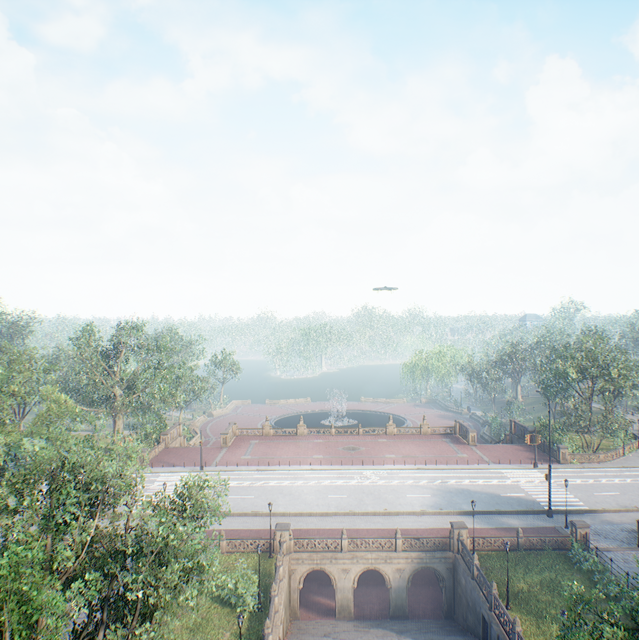
\includegraphics[width=\textwidth]{s2d_input.png}
		\caption{Input image.}
	\end{subfigure}
	\hfill
	\begin{subfigure}[b]{0.4\textwidth}
		\centering
		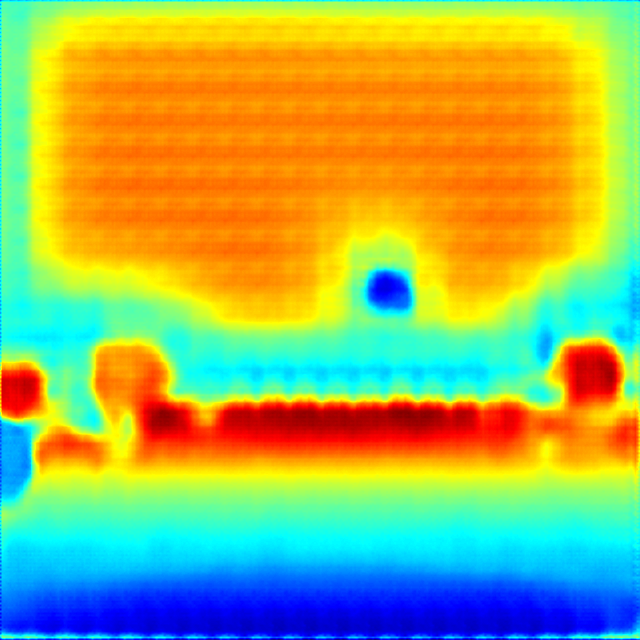
\includegraphics[width=\textwidth]{raws2d_output.png}
		\caption{Output depthmap.}
	\end{subfigure}
	\hfill
	\begin{subfigure}[b]{0.4\textwidth}
		\centering
		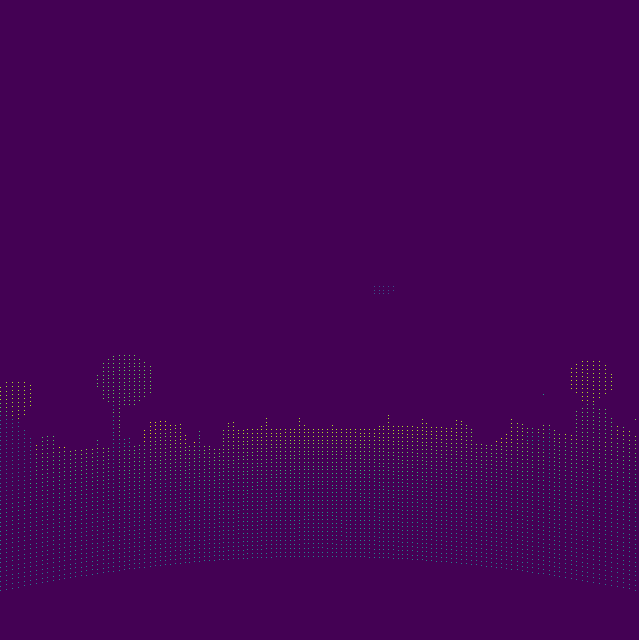
\includegraphics[width=\textwidth]{s2d_all.png}
		\caption{All depthmap points.}
	\end{subfigure}
	\hfill
	\begin{subfigure}[b]{0.4\textwidth}
		\centering
		
\includegraphics[width=\textwidth]{s2d_select.png}
		\caption{Selected depthmap points.}
	\end{subfigure}
	\caption{Sparse-to-dense training.}
	\label{fig:s2d_tr}
\end{figure}\\
\\
Sparse-to-dense modified is another approach used in this thesis. It uses the dense depthmap outputted from the trained Sparse-to-dense network and a sparse depthmap and further filters the dense one. At each pixel of the dense depthmap if there exists a known depth value in sparse depthmap within the range of 3 pixels, the dense depthmap value is kept. Otherwise, the value is overwritten to $-1.0$. The example output of Sparse-to-dense modified can be seen in \autoref{fig:s2d_mod}.
\begin{figure}
	\centering
	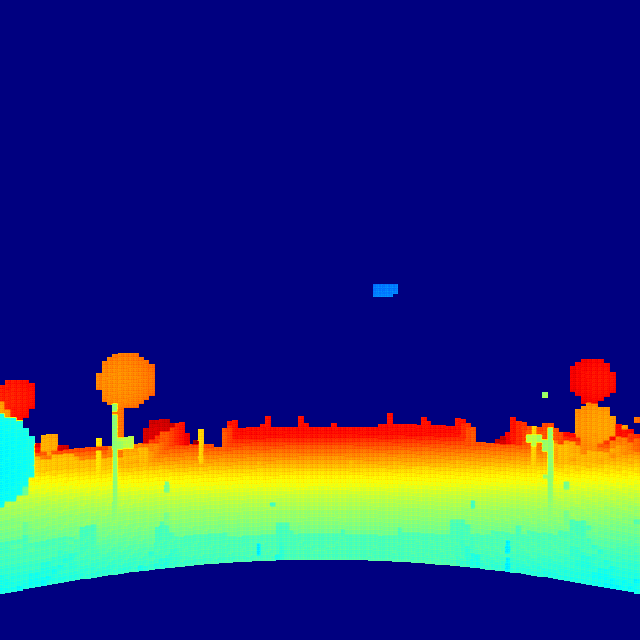
\includegraphics[width=5cm]{sparse2dense_filter.png}
	\caption{Applied filter on Sparse-to-dense output.}
	\label{fig:s2d_mod}
\end{figure}
\section{YOLOv3} \label{s:2.2}
You Only Look Once (YOLO) is a convolutional neural network model used mainly for object detection and recognition \cite{redmon2016look}. The main advantage is its simplicity in comparison to similar convolutional neural networks, resulting in faster detection speeds. The network belongs to the state-of-the-art convolutional neural networks for object detection and recognition. The version used in this work is the third version, called YOLOv3\cite{redmon2018yolov3}. YOLOv3 takes $n$-channel images as the input. Each of the detection layers outputs three bounding boxes for each of the cells. The backbone called Darknet53 consists of 53 convolutional layers. The original detector consists of 3 detection layers each responsible for detecting objects of various sizes as shown in \autoref{fig:yolov3_model}. 
\begin{figure}
	\centering
	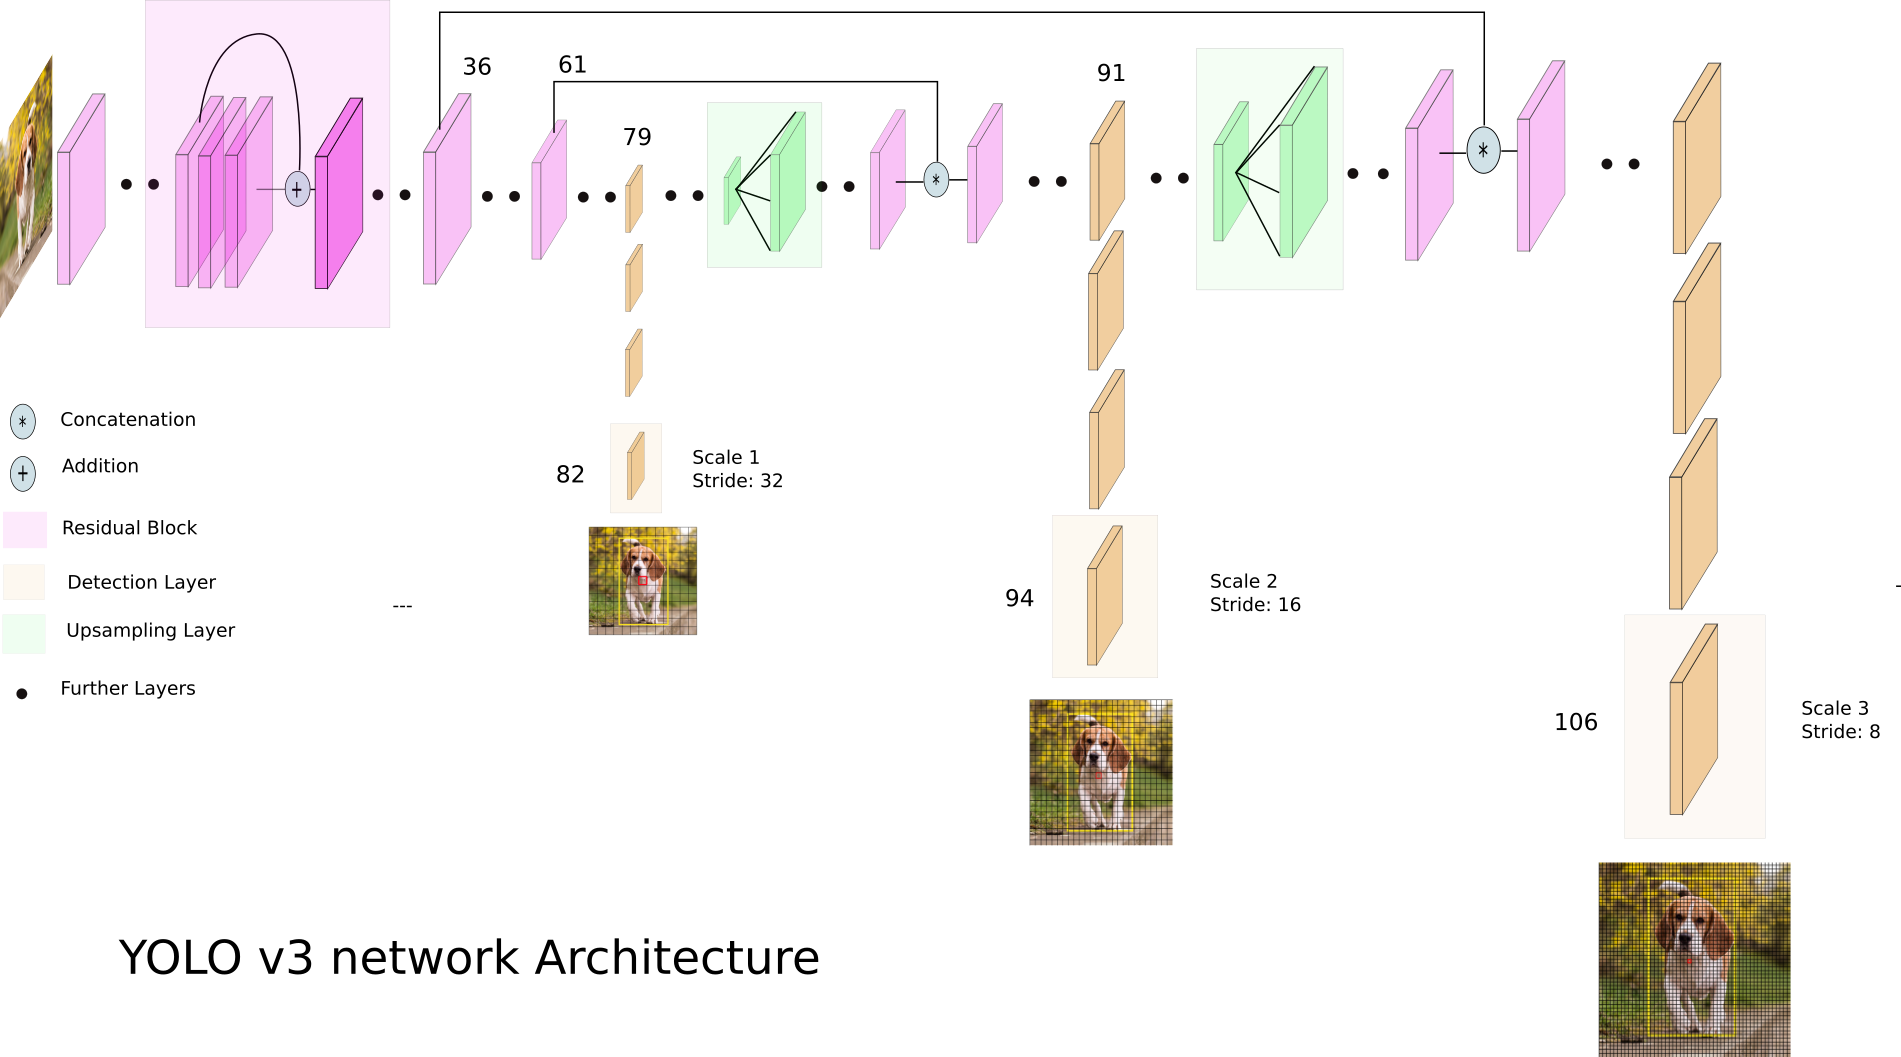
\includegraphics[width=\textwidth]{yolov3_model.png}
	\caption[YOLOv3 network architecture.]{YOLOv3 network architecture\footnotemark.}
	\label{fig:yolov3_model}
\end{figure}
\footnotetext{\url{https://towardsdatascience.com/yolo-v3-object-detection-53fb7d3bfe6b}}
At each detection layer, the image is divided into multiple grid cells, where each grid cell detects three bounding boxes. The content of one bounding box is as follows:
\begin{itemize}
	\item $t_x, t_y, t_w, t_h$ are bounding box coordinates,
	\item $p_O$ is objectness score,
	\item $p_c$ is class score for each class in the dataset.
\end{itemize}
The bounding box $t_x$ and $t_y$ coordinates are relative to the upper-left corner of its respective cell, while $t_w$ and $t_h$ are relative to one of the anchors. Anchors are pre-defined default bounding box sizes and can be modified before training. To transform these bounding box coordinates to be relative to the image the following transformation is applied:
\begin{equation}\label{bbox}
	\begin{aligned}
		b_x&=\sigma(t_x)+c_x,\\
		b_y&=\sigma(t_y)+c_y,\\
		b_w&=p_{w}e^{t_w},\\
		b_h&=p_{w}e^{t_h},
	\end{aligned}
\end{equation}
where
\begin{itemize}
	\item $\sigma(x)$ is a sigmoid function, defined as $\sigma(x)=\frac{1}{1+e^{-x}}$,
	\item $c_x, c_y$ are grid cells offsets from the top left corner of the image,
	\item $p_w, p_h$ are the anchor's width and height, respectively,
	\item $b_x, b_y, b_w, b_h$ are the bounding box coordinates relative to the image size.
\end{itemize}
The loss function used during the training is the sum squared error loss or $L_2$ error described as follows:
\begin{equation}
	L_2=\sum(\mathbf{\hat{t}}-\mathbf{t})^2,
\end{equation}
where
\begin{itemize}
	\item $\mathbf{\hat{t}}$ is a vector of the predicted bounding box coordinates,
	\item $\mathbf{t}$ is a vector of the ground truth bounding box coordinates which can be obtained by inverting the transformation in eq.~\eqref{bbox}.
\end{itemize}
\section{Image inpainting method based on the Fast Marching Method} \label{inpainting}
Image inpainting is a method used for reconstructing missing values in the image. One such method based on \cite{cite:5} called the Image inpainting method based in the Fast Marching Method was used in this thesis and is described in this section. This method is utilized in this thesis for densing a sparse depthmap. A sparse depthmap is provided as the input and the output is dense depthmap. The same method can be extended for RGB images, but is not needed for this thesis.\\
\\
The depth value of a pixel to be inpainted is determined by the known neighbouring pixel values. To compute a depth value from one close pixel the following formula is used:
\begin{equation} \label{eq:1}
	I_q(\mathbf{p})=I(\mathbf{q})+\mathbf{\nabla I(q)}\cdot(\mathbf{p}-\mathbf{q}),
\end{equation}
where:
\begin{itemize}
	\item $\mathbf{q}$ is a vector of pixel coordinates with a known depth value,
	\item $\mathbf{p}$ is a vector of pixel coordinates with an unknown depth value,
	\item $I(\mathbf{x})$ is a depth value at pixel coordinates $\mathbf{x}$,
	\item $\mathbf{\nabla I(x)}$ is a gradient vector at pixel coordinates $\mathbf{x}$.
\end{itemize}
\begin{figure}
	\centering
	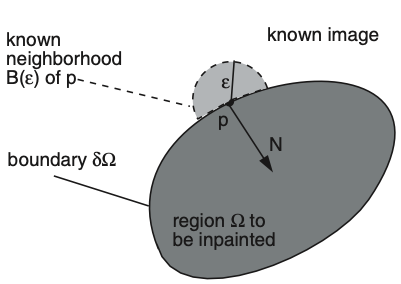
\includegraphics[width=9cm]{inpaint_principle.png}
	\caption[Inpainting principle.]{Inpainting principle. Image from: \cite{cite:5}}
	\label{fig:inpaint_schema}
\end{figure}
To get a final value for the unknown pixel, the Equation \eqref{eq:1} is applied on all known pixels in a specified region $B_{\varepsilon}(\mathbf{p})$ from the unknown pixel as can be seen in  \autoref{fig:inpaint_schema}. The resulting function can be expressed as:
\begin{equation}\label{inpaint_eq}
	I(\mathbf{p})=\frac{\sum_{\mathbf{q}\in B_{\varepsilon}(\mathbf{p})}w(\mathbf{p},\mathbf{q})I_{\mathbf{q}}(\mathbf{p})}{\sum_{\mathbf{q}\in B_{\varepsilon}(\mathbf{p})}w(\mathbf{p},\mathbf{q})},
\end{equation}
where $w(\mathbf{p},\mathbf{q})$ is a weighting function designed for propagating sharpness of the image and is obtained as the product of the following expressions:
\begin{equation}
	\begin{aligned}
		dir(\mathbf{p},\mathbf{q})&=\frac{\mathbf{p}-\mathbf{q}}{||\mathbf{p}-\mathbf{q}||}\cdot\mathbf{N(p)},\\
		dst(\mathbf{p},\mathbf{q})&=\frac{1}{||\mathbf{p}-\mathbf{q}||^2},\\
		lev(\mathbf{p},\mathbf{q})&=\frac{1}{1+|T(\mathbf{p})-T(\mathbf{q})|},
	\end{aligned}
\end{equation}
where
\begin{itemize}
	\item $\mathbf{N(x)}$ is a normal vector of the boundary to be inpainted at pixel $\mathbf{x}$,
	\item $T(\mathbf{x})$ is distance of pixel $\mathbf{x}$ to the inpainting boundary.
\end{itemize}
Eq.~\eqref{inpaint_eq} is iteratively applied to all pixels on the inpainting boundary and advances inside the region to be inpainted until the whole region has been filled. This is implemented via the Fast Marching Method algorithm. Example results of inpainting method can be seen in \autoref{fig:inpaint_ex}.
\begin{figure}
	\caption[Example of the inpainting technique.]{Example of the inpainting technique. Image from: \cite{cite:5}.}
	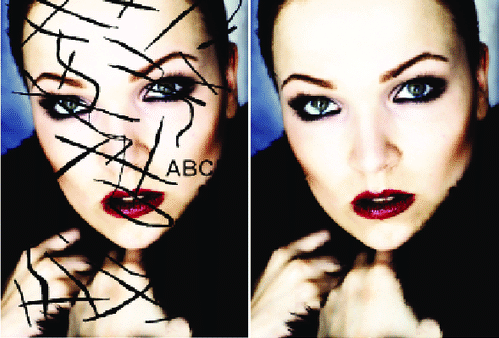
\includegraphics[width=10cm]{inpaint_example.png}
	\centering
	\label{fig:inpaint_ex}
\end{figure}
The algorithm is provided in the OpenCV Python library\footnote{\url{https://docs.opencv.org/4.x/d7/d8b/group__photo__inpaint.html}}.  The results were processed with the same filtering method as for the results of Sparse-to-dense modified method. For further training, only the filtered depth map was used. The results of this approach can be seen in \autoref{fig:inpaint_results}.
\begin{figure}
	\centering
	\begin{subfigure}[b]{0.3\textwidth}
		\centering
		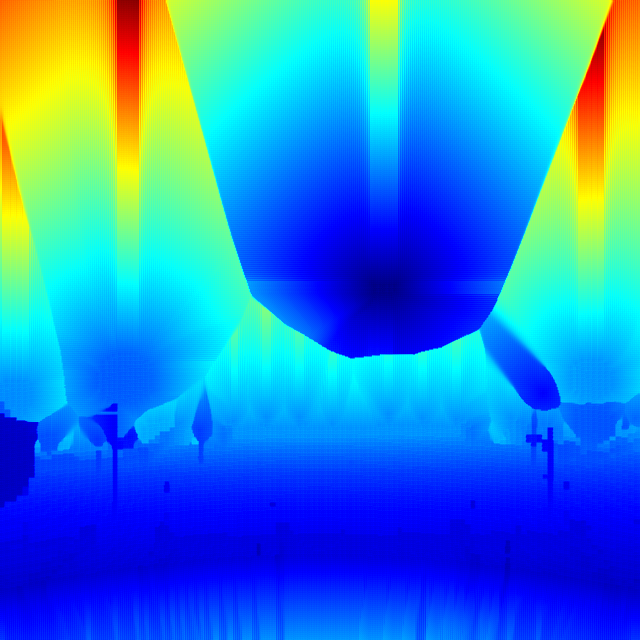
\includegraphics[width=\textwidth]{raw_inpaint.png}
		\caption{Non filtered result.}
	\end{subfigure}
	\hfill
	\begin{subfigure}[b]{0.3\textwidth}
		\centering
		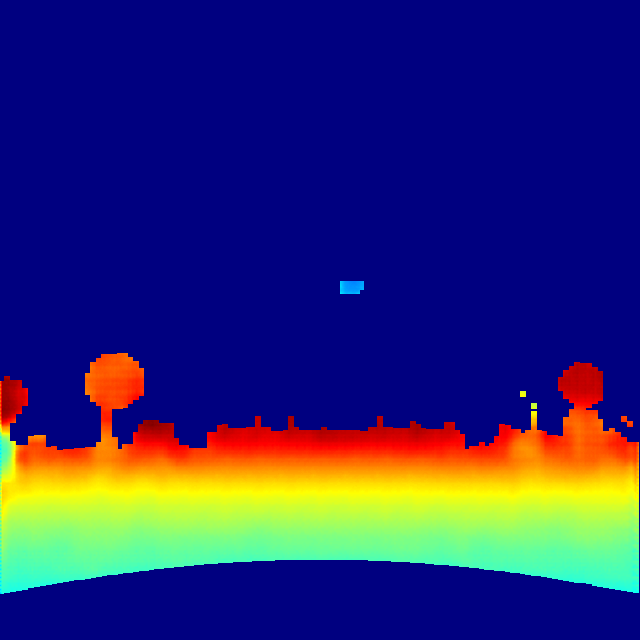
\includegraphics[width=\textwidth]{inpaint.png}
		\caption{Filtered result.}
	\end{subfigure}
	\caption{Inpaint results.}
	\label{fig:inpaint_results}
\end{figure}
\section{Coordinate systems}
To correctly label the data for training, a position of the target drone in relation to the sensor mounted on the observer drone is required. The AirSim API returns the position of each drone in respect to their starting points. The starting point is a point where the drone spawns in the map. Therefore, a transformation from the starting point of the target drone to the camera mounted on the observer is required. This transformation is obtained as:
\begin{equation}
	\textbf{T}=\textbf{T}_{o}^{c}\textbf{T}_{os}^{o}\textbf{T}_{ts}^{os},
\end{equation}
where
\begin{itemize}
	\item $\textbf{T}_{ts}^{os}$ is a transformation from the starting point of the target drone to the starting point of the observer drone,
	\item $\textbf{T}_{os}^{o}$ is a transformation from the starting point of the observer drone to the body of the observer drone,
	\item $\textbf{T}_{o}^{c}$ is a transformation from the body of the first drone to the cameras coordinate system.
\end{itemize}
\begin{figure}
	\centering
	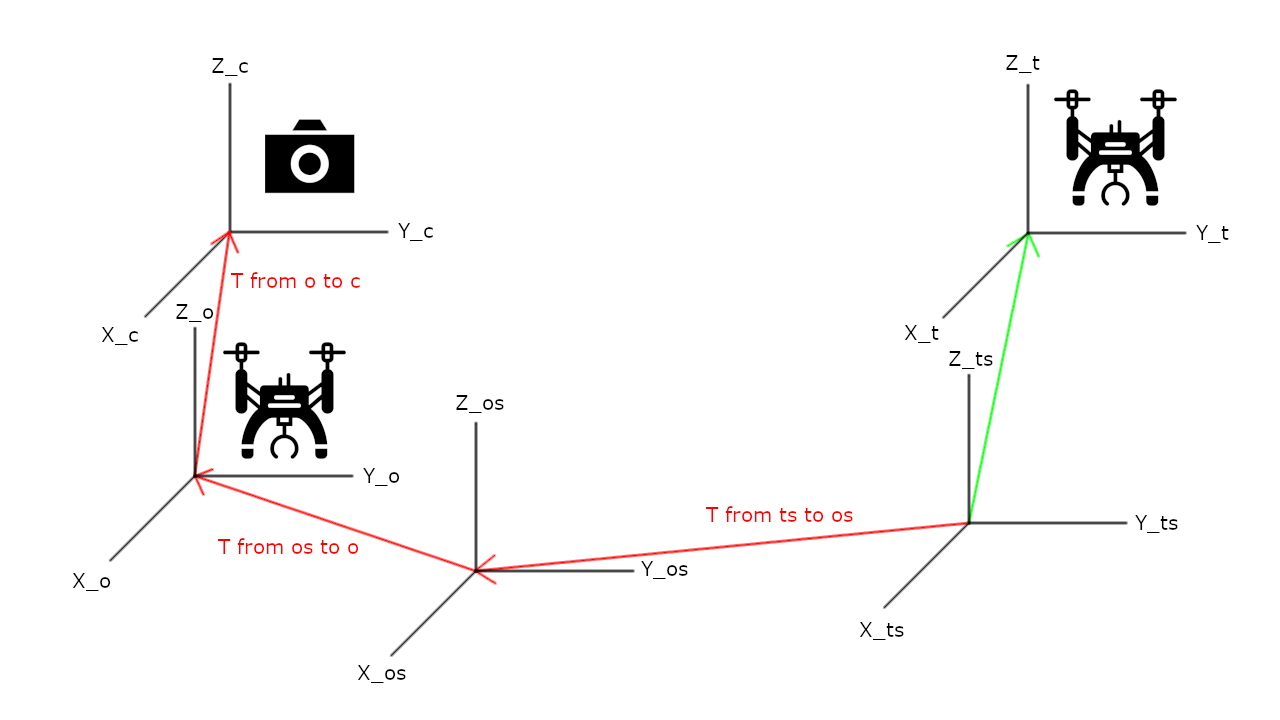
\includegraphics[width=\textwidth]{coord_schema.png}
	\caption{Visualization of transformation.}
	\label{fig:trans}
\end{figure}
The homogeneous transformation matrix $\textbf{T}$ is generally described as:
\begin{equation}
	\textbf{T}=\begin{bmatrix}
		\textbf{R} & \textbf{p}\\
		\textbf{0}^T & 1
	\end{bmatrix},
\end{equation}
where
\begin{itemize}
	\item $\textbf{R}$ is a 3x3 rotation matrix,
	\item $\textbf{p}$ is a 3x1 translation column vector,
	\item $\textbf{0}^T$ is a 1x3 row vector of zeros.
\end{itemize}
To transform a location of the drone represented by vector $\mathbf{v_{ts}}$ into the coordinate system of the camera, as can be seen in \autoref{fig:trans}, the following transformation is applied:
\begin{equation}
	\mathbf{v_c}=\mathbf{T}\mathbf{v_{ts}}.
\end{equation}
\section{Camera Model} \label{sec:camera-model}
For the creation of the bounding boxes used for training of the neural networks and for projecting the LiDAR pointcloud to a depthmap, a transformation from the coordinate system of the camera to the pixel values of the image is required. For this task, a pinhole camera model is used as seen in \autoref{fig:pinhole}.
\begin{figure}
	\centering
	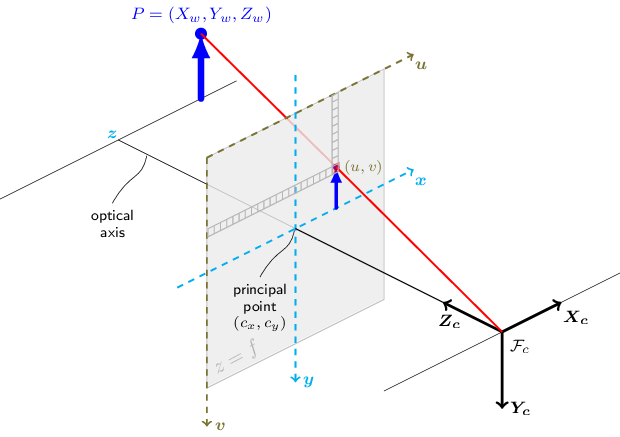
\includegraphics[width=\textwidth]{pinhole_camera_model.png}
	\caption[Pinhole camera model.]{Pinhole camera model\footnotemark.}
	\label{fig:pinhole}
\end{figure}
The transformation is defined as:
\begin{equation} \label{eq:2}
	\begin{bmatrix}
		u\\
		v
	\end{bmatrix}=
	\begin{bmatrix}
		f\frac{X_c}{Z_c}+c_x\\
		f\frac{Y_c}{Z_c}+c_y
	\end{bmatrix},
\end{equation}
where
\begin{itemize}
	\item $u$ and $v$ are pixel coordinate values on the image,
	\item $X_c$, $Y_c$, $Z_c$ are coordinate values of a point in the coordinate system of the camera,
	\item $f$ is the focal length of the camera,
	\item $c_x$,$c_y$ are pixel coordinates of the center of the image plane.
\end{itemize}
The pinhole camera model is only an idealization of a real life camera and no lens distortion is considered. The AirSim simulator simulates an ideal pinhole camera so no other processing was done for the purposes of this thesis.
\footnotetext{\url{https://docs.opencv.org/4.x/d9/d0c/group__calib3d.html}}
\section{Training and testing dataset} \label{s:2.6}
The dataset in this thesis was used for training and testing of all used approaches for drone detection. It can be generated in two ways. The first is real-life drone shots mixed with pointclouds from LiDAR mounted on top of a drone. The second is generating a dataset using a realistic virtual environment where a drone, camera and LiDAR are being emulated very close to their real-life counterparts. An advantage to this approach is that a great variety of environments can be chosen a lot of them often inaccessible otherwise (power plant, airport, snowy mountains out of season etc.). Therefore, this approach was chosen for the task.
\subsection{Unreal Engine}
Unreal Engine is a software tool used for creating realistic 3D environments, most often used as a video game engine. It is written in C++ and open-source supporting a variety of pre-built environments and assets. Example of an Unreal Engine interface can be seen in \autoref{fig:ue_int}. For this work, three different environments were used for the creation of the dataset, that are illustrated in \autoref{fig:ue_env}:
\begin{itemize}
	\item City Park Environment Collection (2256 samples taken),
	\item Automotive Winter Scene (1813 samples taken),
	\item Downtown West Modular Pack (1251 samples taken).
\end{itemize}
\begin{figure}
	\centering
	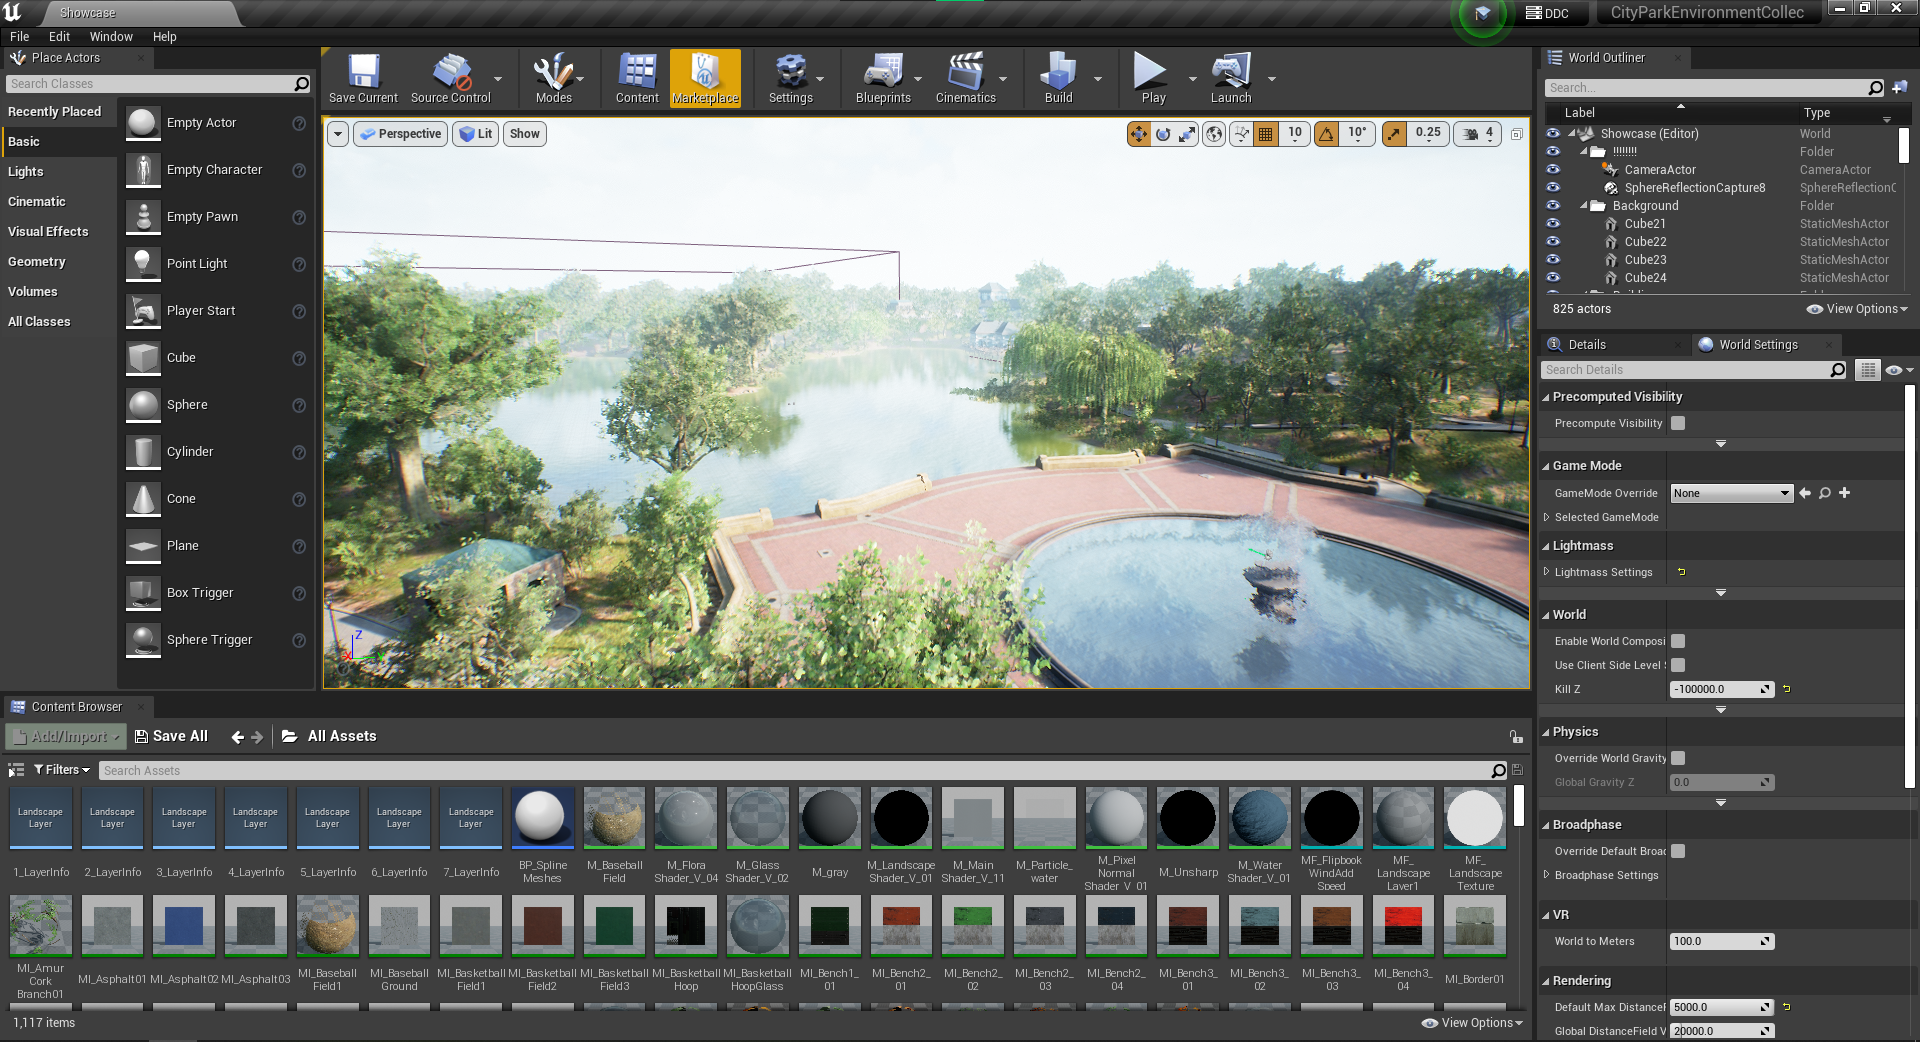
\includegraphics[width=\textwidth]{unreal_ui.png}
	\caption{Unreal Engine user interface.}
	\label{fig:ue_int}
\end{figure}
\begin{figure}
	\centering
	\begin{subfigure}[b]{0.3\textwidth}
		\centering
		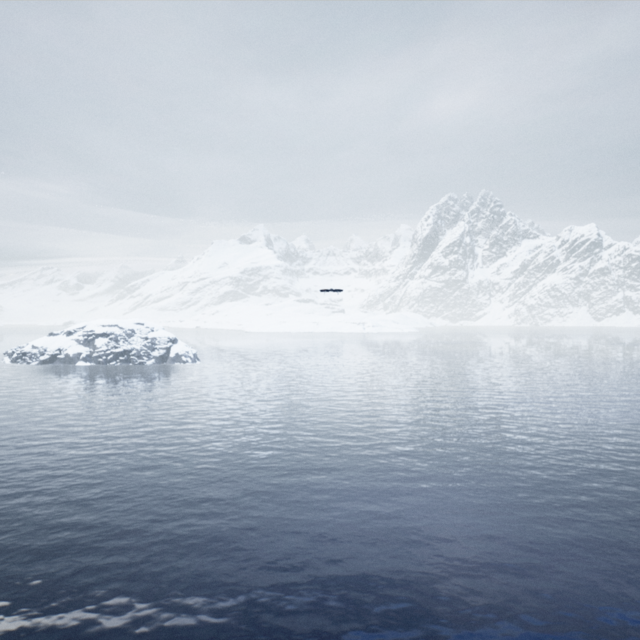
\includegraphics[width=\textwidth]{snow_rgb.png}
		\caption{Automotive Winter Scene.}
	\end{subfigure}
	\hfill
	\begin{subfigure}[b]{0.3\textwidth}
		\centering
		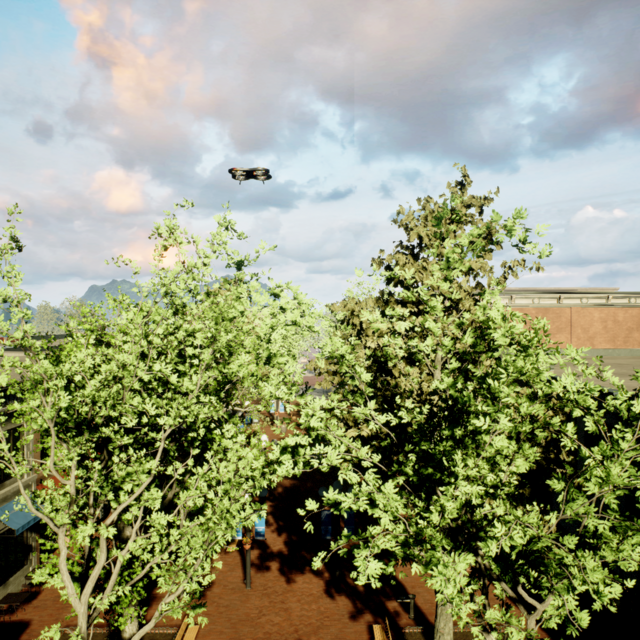
\includegraphics[width=\textwidth]{city_rgb.png}
		\caption{City Park Environment Collection.}
	\end{subfigure}
	\hfill
	\begin{subfigure}[b]{0.3\textwidth}
		\centering
		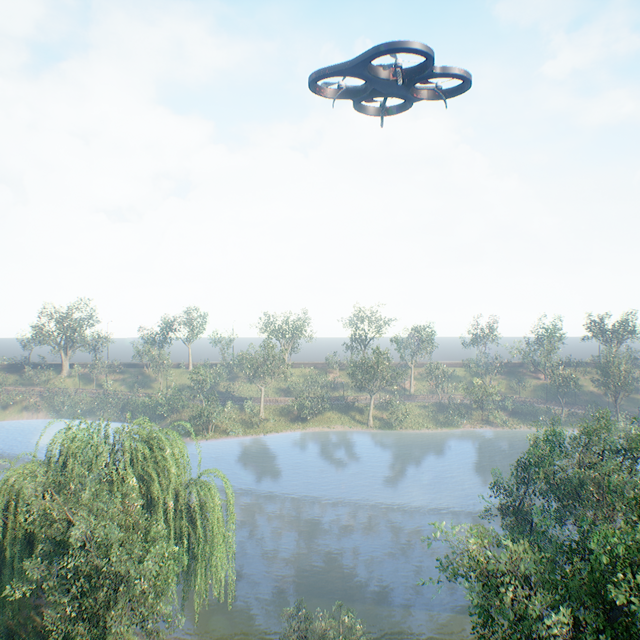
\includegraphics[width=\textwidth]{park_rgb.png}
		\caption{Downtown West Modular Pack.}
	\end{subfigure}
	\caption{Sample photos from each environment.}
	\label{fig:ue_env}
\end{figure}
Together, 5320 pictures and labels were generated using two drones. The observer drone was equipped with an RGB camera and the LiDAR sensor and was taking pictures using the camera and pointclouds from the LiDAR. The Parrot AR.Drone 2.0 shown in \autoref{fig:parrot} was used as a model for the drone detection target.
\begin{figure}
	\centering
	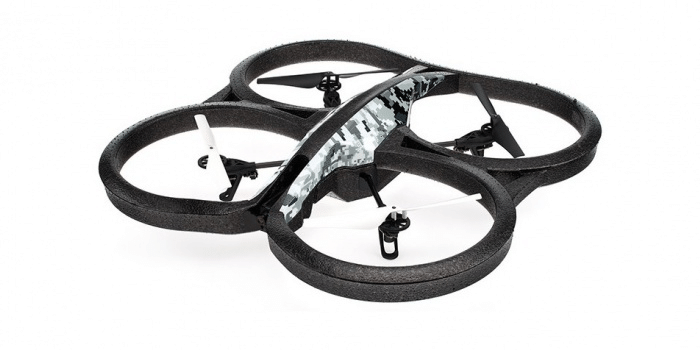
\includegraphics[width=\textwidth]{parrot.png}
	\caption[Parrot AR.Drone 2.0.]{Parrot AR.Drone 2.0. Image taken from \cite{parrot}.}
	\label{fig:parrot}
\end{figure}
\subsection{AirSim}
An open-source plugin for Unreal Engine called AirSim was used for the generation of the dataset. It simulates realistic flight motions of drones as well as seven types of sensors, including RGB cameras and LiDARs, which are the types used for this thesis. AirSim supports both a C++ API as well as a Python API, the latter of which was used for controlling motion of the observer and target drones and capturing the dataset. The location of the second drone was generated through API call, which produces a location of the drone in local coordinates relative to its starting point, which is later transformed to the local coordinates of the first drone carrying the LiDAR and RGB sensors using eq. \eqref{eq:2}. The ground-truth bounding boxes required for the training of the convolutional neural network were generated the same way but instead of the target's center, corner points of the 3D bounding box were transformed using eq.\eqref{eq:2}. The bounding box dimensions were set to $\SI{0.6}{\metre} \times \SI{1.0}{\metre} \times \SI{0.3}{\metre}$. The LiDAR pointcloud was generated via an API call, which returns a set of 3D coordinates of the points measured by the sensor in a coordinate frame of the observer drone. Therefore transformation \eqref{eq:2} was utilized. The capturing drone travelled on each map on a 3D cube grid.
\section{Training}
For training and testing purposes, 5320 samples were taken using the AirSim simulator. Each sample consists of:
\begin{itemize}
	\item a $640px \times 640px$ RGB image from the camera,
	\item a $640px \times 640px$ sparse depth image from the LiDAR sensor,
	\item a label file containing coordinates of the ground-truth bounding boxes.
\end{itemize}
This dataset was split into 3662 training, 407 validation, 1251 testing samples.
\subsection{Sparse-to-dense}
The Sparse-to-dense neural network was trained using RGB images and sparse depthmaps. The training was done for 15 epochs using a batch size of 8. The backbone was Resnet18 and the decoder was set to Deconv3 as described in \autoref{s2d}. According to the authors of Sparse-to-dense \cite{ma2018sparsetodense} this provided the best overall results. A processing algorithm was applied to the output depth map, further filtering points that were not in the vicinity of the ground truth depth points. Both filtered and unfiltered depth maps were used for further training and testing to clarify their overall impact.
\subsection{YOLOv3}
The following parameters were used for training all the methods:
\begin{itemize}
	\item number of epochs was set to 15,
	\item batch size was set to 64,
	\item learning rate was set to 0.001.
\end{itemize}
A PyTorch implementation of YOLOv3 was used for training\footnote{\url{https://github.com/eriklindernoren/PyTorch-YOLOv3}}. Further modifications were made. The original implementation of YOLOv3 supports 3-channel RGB images as inputs. For the sake of this work, an RGBD input option using the H5 file system was implemented. The dataset consisted of drones of various sizes ranging from very small (few pixels) to very large closeups. Therefore, 5 detection layers were implemented instead of the original 3. The addition of two more detection layers provide finer cell division when determining the location and the size of the bounding box, which helps detecting smaller objects. The sample outputs can be seen in \autoref{fig:yolo_out}.
\begin{figure}
	\centering
	\begin{subfigure}[b]{0.4\textwidth}
		\centering
		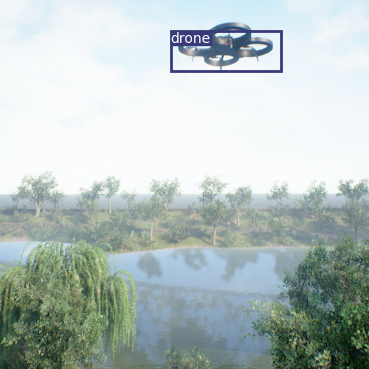
\includegraphics[width=\textwidth]{02167.png}
	\end{subfigure}
	\hfill
	\begin{subfigure}[b]{0.4\textwidth}
		\centering
		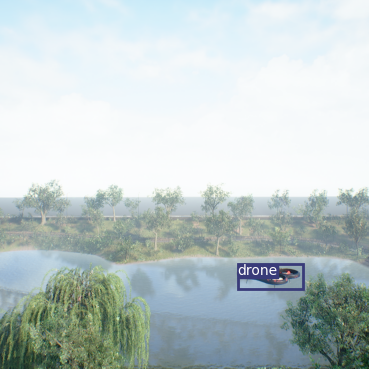
\includegraphics[width=\textwidth]{02665.png}
	\end{subfigure}
	\caption{Sample YOLOv3 outputs.}
	\label{fig:yolo_out}
\end{figure}
\begin{figure}
	\centering
	\begin{subfigure}[b]{0.7\textwidth}
		\centering
		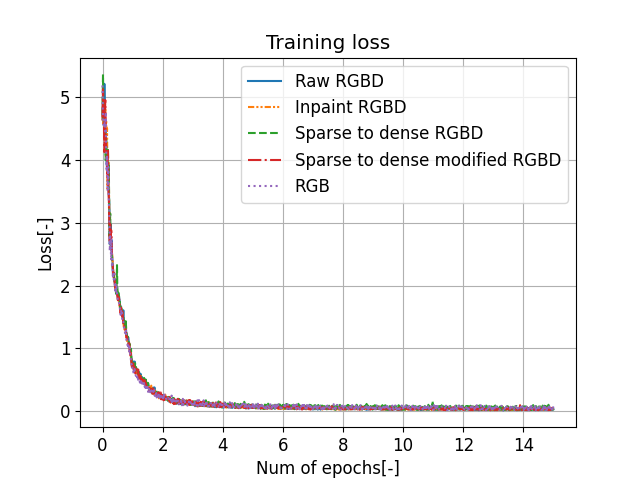
\includegraphics[width=\textwidth]{train_loss.png}
	\end{subfigure}
	\hfill
	\begin{subfigure}[b]{0.7\textwidth}
		\centering
		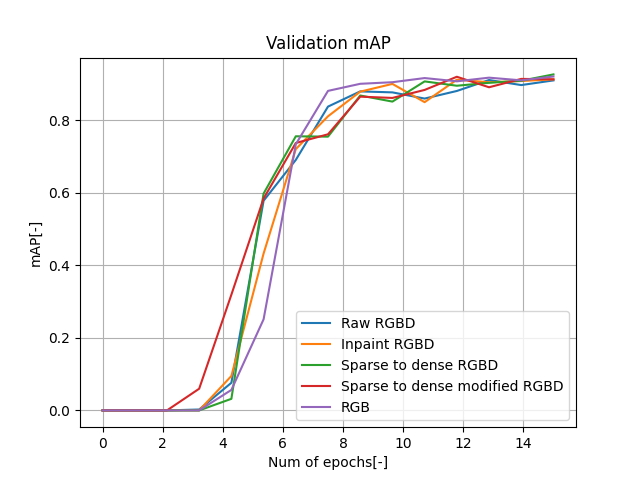
\includegraphics[width=\textwidth]{validation_mAP.png}
	\end{subfigure}
	\caption{Comparison of the training loss and validation AP scores for the different methods during training}
	\label{fig:yolo_res}
\end{figure}
During training, the validation AP followed the training loss and started converging after around the 8th epoch, as is apparent from the graphs in \autoref{fig:yolo_res}. Considering this, the chosen weights ensured that the network does not overfit the training and validating dataset. \autoref{table:weights} shows selected weights for each method.
\begin{table}
\begin{tabular}{|c|c|c|c|c|c|}
	\hline
	& \begin{tabular}[c]{@{}c@{}}RGB\\ (baseline)\end{tabular} & \begin{tabular}[c]{@{}c@{}}Inpaint\\ RGBD\end{tabular} & \begin{tabular}[c]{@{}c@{}}Sparse-to-dense\\ RGBD\end{tabular} & \begin{tabular}[c]{@{}c@{}}Sparse-to-dense\\ modified RGBD\end{tabular} & \begin{tabular}[c]{@{}c@{}}Raw\\ RGBD\end{tabular} \\ \hline
	\begin{tabular}[c]{@{}c@{}}Weights\\ {[}number of training epochs{]}\end{tabular} & 8                                                        & 9                                                      & 11                                                             & 12                                                                      & 9                                                  \\ \hline
\end{tabular}
	\caption{Chosen weights.}
	\label{table:weights}
\end{table}
\chapter{Results}
After the training was completed, the different metrics on the validation dataset were compared. These metrics include:
\begin{itemize}
	\item precision,
	\item recall,
	\item Intersection over Union (IoU),
	\item Average Precision (AP).
\end{itemize}
These metrics are given by the following formulas:
\begin{equation}
	\begin{aligned}
		precision &= \frac{\text{True Positives}}{\text{True Positives} + \text{False Positives}},\\
		recall &= \frac{\text{True Positives}}{\text{True Positives} + \text{False Negatives}},\\
		IoU &= \frac{\text{Area of overlap of two bounding boxes}}{\text{Area of union of two bounding boxes}}.\\
	\end{aligned}
\label{eq:metrics}
\end{equation}
where:
\begin{itemize}
	\item $N$ is number of classes.
\end{itemize}
$AP$ is calculated by plotting Precision against Recall obtained in eq. \eqref{eq:metrics} and calculating the area under the resulted curve.\\
\\
After the weights were chosen, the network was validated on the test dataset. The confidence threshold was chosen to be $0.2$ and IoU threshold was set to $0.5$. These settings showed best overall results for all the methods.
\begin{table}
\begin{tabular}{|c|c|c|c|c|c|}
	\hline
	Results   & \begin{tabular}[c]{@{}c@{}}RGB\\ (baseline)\end{tabular} & \begin{tabular}[c]{@{}c@{}}Inpaint\\ RGBD\end{tabular} & \begin{tabular}[c]{@{}c@{}}Sparse-to-dense\\ RGBD\end{tabular} & \begin{tabular}[c]{@{}c@{}}Sparse-to-dense\\ modified RGBD\end{tabular} & \begin{tabular}[c]{@{}c@{}}Raw\\ RGBD\end{tabular} \\ \hline
	AP       & 0.41                                                     & 0.46                                                   & 0.36                                                           & 0.43                                                                    & \textbf{0.48}                                      \\ \hline
	precision & 0.79                                                     & 0.89                                                   & \textbf{0.92}                                                  & 0.60                                                                    & 0.59                                               \\ \hline
	recall    & 0.48                                                     & 0.48                                                   & 0.37                                                           & 0.48                                                                    & \textbf{0.53}                                      \\ \hline
	IoU       & 0.83                                                     & \textbf{0.84}                                          & \textbf{0.84}                                                  & 0.83                                                                    & 0.79                                               \\ \hline
\end{tabular}
	\caption{Comparison of different metrics on the testing dataset for the evaluated detection methods}
	\label{tab:res}
\end{table}
\begin{figure}
	\centering
	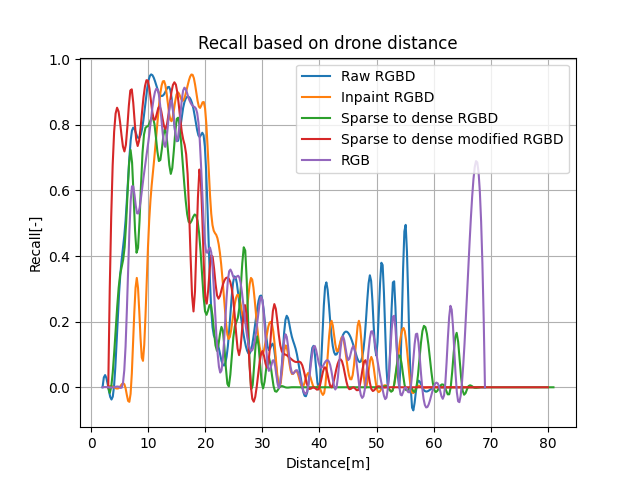
\includegraphics[width=\textwidth]{recall_distance.png}
	\caption{Recall over distance of the drone.} \label{fig:recall_distance}
\end{figure}
From the results presented in Table \ref{tab:res}, Raw RGBD offers the best improvement in terms of AP by 7\% when compared to the baseline RGB-only method. Every method except Sparse-to-dense RGBD offers some improvement in terms of AP over the baseline. In terms of precision, Sparse-to-dense RGBD and Inpaint RGBD offer an improvement over RGB-only by 13\% and 10\% respectively. Other methods namely Raw RGBD and modified Sparse-to-dense RGBD offer a decrease of 20\% and 19\% respectively. When it comes to the recall, not a big improvement is made. The best method is Raw RGBD with an increase of 5\% in comparison to RGB-only. Sparse-to-dense RGBD suffers a decrease of 11\% in comparison to RGB-only, while the remaining methods are unchanged. This can be observed in \autoref{fig:recall_distance} where all methods perform the best in the range from 4 to 19 meters reaching a maximum recall of around 0.95. Modified Sparse-to-dense RGBD offers the highest recall in around 4 meters but starts to fall after 18 meters. Raw RGBD shows a few spikes in the range from around 48 to 55 meters, the highest reaching 0.5 recall. RGB-only shows a spike at around 67 meters with a recall of around 0.7. In terms of the IoU, all methods perform very similarly with best-performing methods Inpaint RGBD and Sparse-to-dense RGBD showing improvement of 1\%.
\begin{table}
		\begin{tabular}{|c|c|c|c|c|c|}
			\hline
			Speed             & \begin{tabular}[c]{@{}c@{}}RGB\\ (baseline)\end{tabular} & \begin{tabular}[c]{@{}c@{}}Inpaint\\ RGBD\end{tabular} & \begin{tabular}[c]{@{}c@{}}Sparse-to-dense\\ RGBD\end{tabular} & \begin{tabular}[c]{@{}c@{}}Sparse-to-dense\\ modified RGBD\end{tabular} & \begin{tabular}[c]{@{}c@{}}Raw\\ RGBD\end{tabular} \\ \hline
			Duration {[}ms{]} & \textbf{39}                                              & 542                                                    & 67                                                             & 76                                                                      & 61                                                 \\ \hline
		\end{tabular}
	\caption{Average processing duration of all methods.}
	\label{tab:speed}
\end{table}\\
\\
\autoref{tab:speed} presents the total processing durations of the evaluated methods from acquiring the image to providing the detection output. The times shown represent a mean from 1251 test samples. From the results, the 4th channel depth input almost doubles the inference time of YOLOv3, while Sparse-to-dense network alone performs quite fast. The longest time for inference belongs to the Inpaint RGBD method with 0.5424 seconds.\\
\\
Overall Raw RGBD provides an increase in AP and recall in comparison to RGB-only method but suffers a decrease in precision. The inference time is longer, which may prove to be a problem in real-life applications.\\
\\
Inpaint RGBD produces overall better results in every metric compared to RGB-only but suffers heavily in long inference times, making it inappropriate for real-life applications where fast tracking is required.\\
\\
Sparse-to-dense RGBD offers a decrease in AP and recall but provides overall the best precision out of any method tested. Sparse-to-dense network output time is slowing down the inference speed by only a small amount.\\
\\
Sparse-to-dense modified RGBD provides little improvement in terms of AP and suffers a decrease in precision. Out of any other method, it provides the highest recall in close detection distances. The modifying algorithm is responsible for a very little slowdown compared to Sparse-to-dense RGBD.
\chapter{Conclusion}
In this thesis, four different methods of fusion of RGB data with LiDAR data for the purpose of drone detection were proposed and compared to an RGB only method. Virtual environments were used for the generation of the dataset. A detection convolutional neural network was trained from scratch and tested using various metrics that were compared with the RGB-only baseline CNN. The advantage of these methods is that they can be easily implemented on drones already carrying these sensors, or on drones already carrying a LiDAR sensor as RGB camera is lightweight and cheap. Since these methods provide detection of drones, there is no need to rely on pre-existing sensor infrastructure as in the case of absolute localization methods. These methods also do not rely on markers placed on target drones, so they can be used in a wider variety of scenarios, where f.e. the target is an uncooperative drone.\\
\\
The dataset used in this method was generated using a variety of virtual environments as described in \autoref{s:2.6}. The engine used for the creation of the dataset proves to be useful when trying to simulate real-life situations and environments. The main advantage is that environments can be created based on specific drone scenarios, without the need to physically simulate such scenarios. Expanding on the number of different environments and the number of different drone models could be an improvement for the overall generalisation and size of the dataset in future works.\\
\\
The main detection convolutional neural network was described in \autoref{s:2.2}. The network was modified from its original implementation to process RGBD data and to detect smaller objects as flying drones that are farther away are only a few pixels in size. A more specific custom-designed architecture could prove to bring an overall improvement on the problem and should be further studied and compared.\\
\\
Overall, the results show that no single approach excels over others in all tested metrics. In situations where high precision is required, the best method is the one utilizing the Sparse-to-dense preprocessing CNN. It suffers no significant slowdowns in terms of inference time and provides the best precision out of all tested methods. A modified method from \autoref{s2d} proves to provide a higher recall compared to other methods in terms of close distance detection. Compared to other methods, RGB only method provides the most balanced results in all the metrics and the best result in terms of inference speed, making it the best default method for drone detection out of all the tested methods. When it comes to more specific scenarios the fusion of LiDAR and RGB data will excel more.\\
\\
This thesis aimed to compare different approaches of fusion of LiDAR and RGB data and compare them with RGB only method. This assignment was satisfied and proved that some approaches of LiDAR and RGB fusion can have better results in some specific scenarios. The fusion of LiDAR and RGB has got potential for future works and with larger dataset methods tested in this thesis could overall be better then RGB methods.
\bibliographystyle{ieeetr}
\bibliography{ctutest}
\end{document}
